\chapter{Architecture}
\label{chapter:architecture}


Taking into account the goals of this project and all the technology presented so far. Our proposal is the development of a web application that provides communication and collaboration features in real-time.

\section{Requirements}
In a general way our system's goal is to provide a multi-party video and audio conference environment that supports chat, time manipulation, collaborative text edition and hyper-content creation.

%RP isto pode ser muito expandido. Podes começar por descrever os goals (mais alto nível): audio e video conferência multi-party, possibilidade de rever o que foi dito antes, chat, etc etc.
% Só depois traduzes isso em requisitos, tanto funcionais como não funcionais
% Depois apresentas a arquitectura, fazendo um paralelo entre os módulo e escolhas realizadas e quais os requisitos que cada um deles satisfaz. 

For our system, the goals include:

\begin{itemize}
 \item \textbf{Instant Messaging} - Our application must provide a simple way to send instant text messages to the conference participants.
 \item \textbf{Room management} - Conference rooms can be public or private. Public chat rooms are moderated by a group of clients which initially consists only of the room creator. This type of room has no access restrictions by default, but that can be changed by its moderators. Private chat rooms will only be visible to a defined list of clients or can be accessed by clients that have a link for that conference room.
 \item \textbf{Stream Recording} - Ability to recording and playback recorded video including all the hyper-content displayed at that time.
 \item \textbf{Stream Composition} - Our streaming server must support mixing multiple user streams into a single stream. The sound played on clients must be the composed sound of all participants but the video played can be switched to the individual or group view.
 \item \textbf{Time annotations} - Our application must give the possibility to create annotations associated to a specified time and support viewing them on a time-line. 
 \item \textbf{Content Overlay} - Our system must allow users to superimpose hyper-content to video given a range of time. This content can be continuous or discrete and interactive or non interactive.
 \item \textbf{Search} - Unified search every objects related to a conference room such as hyper-content, time annotations and users.
 \item \textbf{Content Sharing} - Our application must have the ability to share files and time links among users.
 \item \textbf{Active talker detection} - The system must enable sound detection for showing the current speaker.
 \item \textbf{Collaboration} - The web application must provide a collaborative text edition tool.
 \item \textbf{QR Code detection} - The system must interpret \emph{QR codes} in order to ease content creation.
 \item \textbf{NAT Traversal} - The system's services must be available to users that are inside a private network.
 \item \textbf{Fault tolerance} - Our system's must use a database that supports data replication.
 \item \textbf{Scalability} - Our system must be horizontally scalable, which means that load must be distributed across web, streaming and database servers.
\end{itemize}

%RP capacidade de lidar com NAT

	Moreover we allow clients to discover chat rooms and other clients by navigating on the web pages provided by our web server. In addition users can create rooms for multi-party audio and video communication communication which is achieved by using \ac{WebRTC}'s \emph{PeerConnection}.
        %RP falas em peerconnection, mas na figura 3.1 apenas há um cliente, o que obviamente impede mostrar a comunicação entre peers.
        %RP acho que podes fazer outro diagrama com a comunicação entre os vários componentes, onde apareceriam vários clientes. A aí indicas o tipo de ligação entre cada par de componentes (HTTP, PeerConnectino, websocket, MediaStream ...)
        
\section{Modules}
In this section we present the several modules that were designed in order com fulfill the set requirements.
	Figure~\ref{fig:modules} presents the structure of our system which was divided into six modules:


\begin{figure}
	\centering
	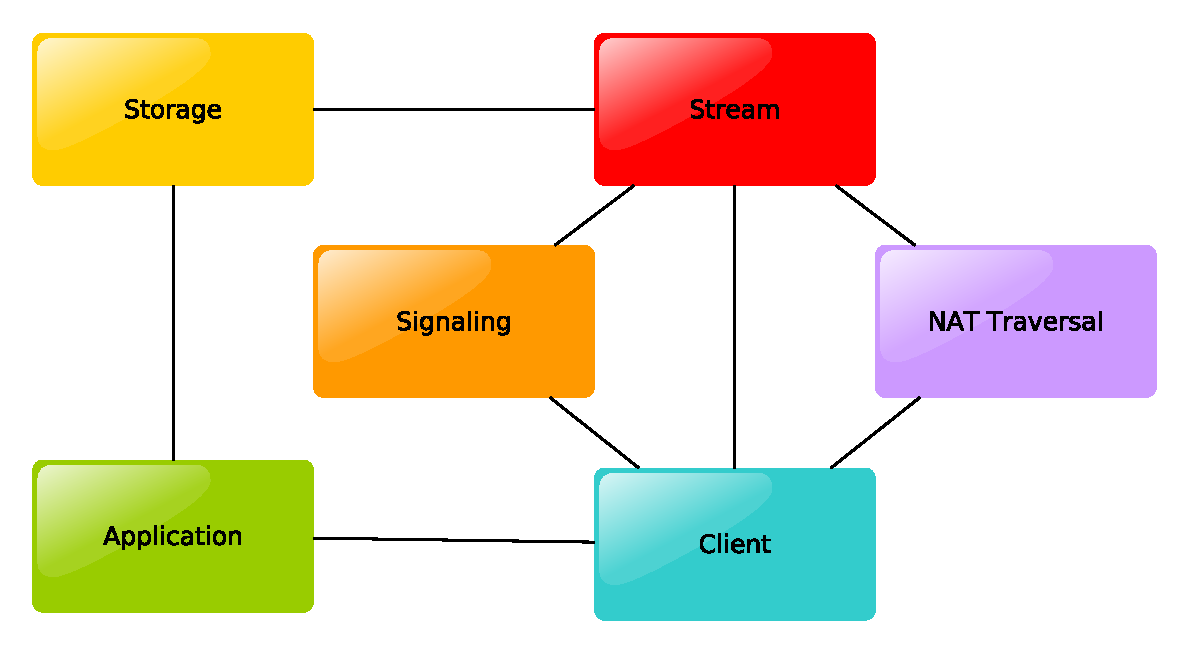
\includegraphics[width=0.8\textwidth]{figures/modules.pdf}
	\caption{System Modules}
    \label{fig:modules}
\end{figure}



\begin{itemize}

\item \textbf{Application module} - responsible for providing information about the relevant modules (\emph{NAT Traversal} and \emph{Signaling}) and user interface to the \emph{Client} in the form of web pages in \ac{HTML} and \emph{JavaScript} libraries through \ac{HTTP}.
 
\item \textbf{Signaling module} - responsible for \emph{Client} and \emph{Stream} coordination which will be performed using \emph{WebSockets}.

 \item \textbf{NAT Traversal module} - \ac{STUN} and \ac{TURN} techniques used by \emph{Client} and \emph{Stream} modules during the \emph{Signaling} phase which ends by establishing the connection between them.

 \item \textbf{Stream module} - responsible to deliver and receive multimedia content from the \emph{Client} using \ac{WebRTC}. 

 \item \textbf{Storage module} - provides two main functionalities: store the model information and media recorded. This is the single module responsible for persistent storage. It stores user and communication data as well as all the data required among user sessions. It is also use to store all the communication streams, so that they can be viewed later.

 \item \textbf{Client module} - responsible for the interaction with the user.

\end{itemize}

%RP Acho que podes escrever muito mais sobre cada componente. Isto está muito curto. Fala de algumas das funções que proporcionam. Vê o que fiz com o Storage Module

%RP também podes fazer um diagrama com vários utilizadores e mostrar quais os streams que vão de e para cada um (mostrar a mistura de som, video, etc).

 
\section{Implementation Proposal}
The infrastructure is composed by: web server, stream server, signaling server, database and video repository.
%RP tens da fazer o paralelo entre isto e os componentes apresentados na secção anterior. O mesmo com a imagem, que parece não estar relacionada. Podes colocar os elementos na mesma posição, ou dentro das caixas da imagem 3.1

\begin{figure}[H]
	\centering
	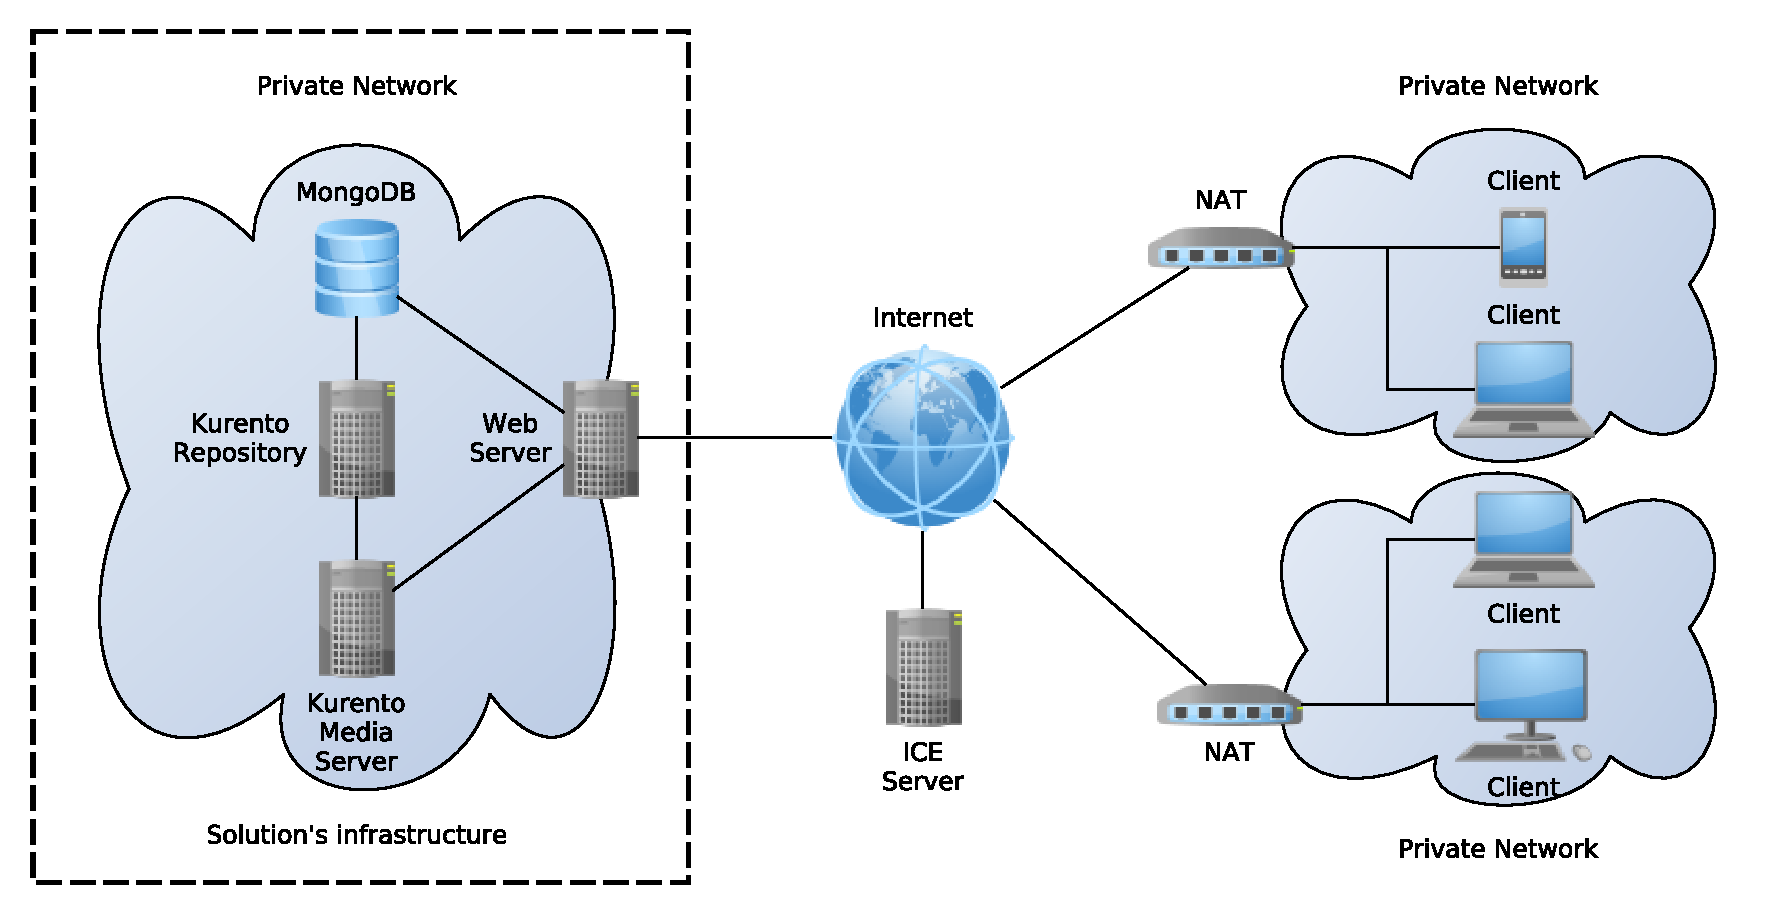
\includegraphics[width=\textwidth]{figures/infrastructure.pdf}
	\caption{System Infrastructure}
\end{figure}

In order to simplify our solution, we propose that the \emph{Application}, \emph{Signaling}, \emph{Stream} and \emph{Storage} modules be implemented within the same server application, so it could be easy to deploy as a single image. To this set of modules, we often call \emph{backend}.

	\subsection{Security and authorization}

Having established that the \emph{backend} modules are placed in the same machine, that helps controlling which resources the client has permission to access as those modules are seen as a private network.
%RP na mesma ``server application'' ou ``machine''? São coisa diferentes! Apresentas vantages de instalar tudo na mesma máquina mas não falas das desvantagens. Menor escalabilidade parece-me ser logo uma delas. Na figura 3.2 aparecem várias máquinas!

To qualify the above we provide public access to \ac{HTTP} server ports, maintaining the access to other components restricted through firewall rules.
%RP qualify?
%RP Imagem com firewall e estes portos? Mas isto já me parece muito detalhe de implementação.
In relation to the database there is no directly access from the outside. All the database information is accessed via our application server which validates the permissions of users on our system.

On the other hand, the access to our streaming servers is also restricted, but clients can connect to them after concluding the signaling phase. This signaling phase may or not proceed in function of the client access permissions. For example, if a user is trying to access a private conference room that he is not a member of nor has an invitation link for, the signaling server refuses to start the signaling phase and the user cannot access the streaming server.

The placement of our streaming servers inside a \ac{NAT} also has an important role with respect to external misuse prevention. Otherwise, placing our streaming servers could allow external clients to perform their own signaling protocol and, as a consequence, use our infrastructure without our consent.

\subsection{Client connections}
	Although the delegation of processing work to clients can improve our system's scalability, we are concerned about using the least resources possible on the client side, as huge resource consumption may drain battery very fast or may even be impossible to run on mobile devices. We are aware that streaming video from clients is already a very intensive task which we cannot avoid but can improve by delegating the most intensive tasks to our servers. 

\begin{figure}
\centering
\begin{minipage}[b]{0.45\linewidth}
	\centering
	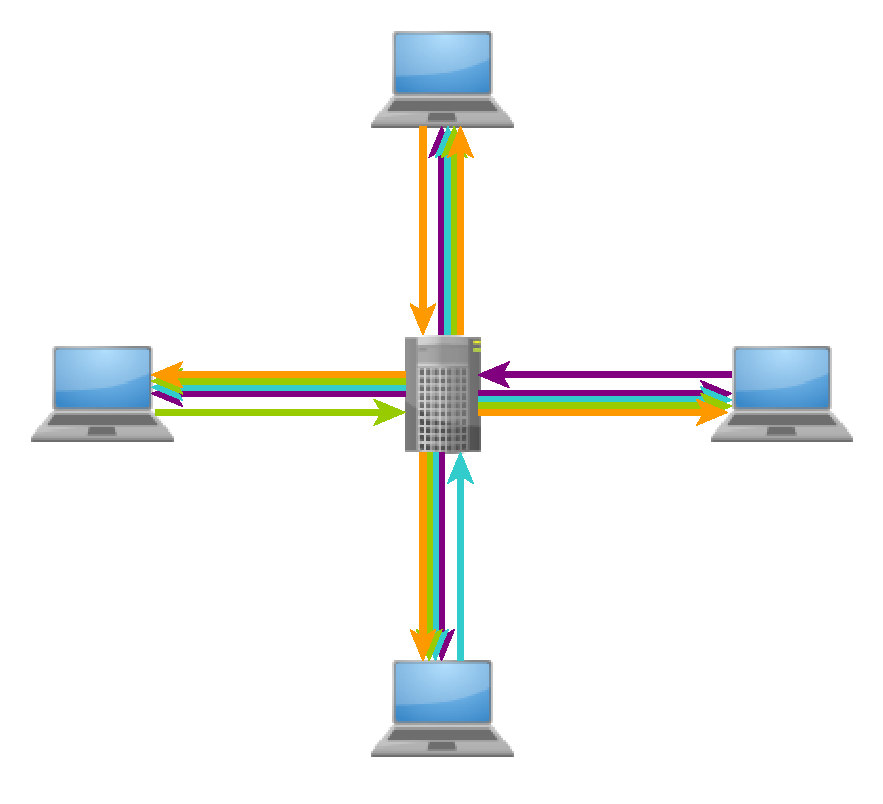
\includegraphics[width=\textwidth]{figures/ccomposite.pdf}
	\caption{Centralized connections}
	\label{fig:central}
\end{minipage}
\quad
\begin{minipage}[b]{0.45\linewidth}
	\centering
	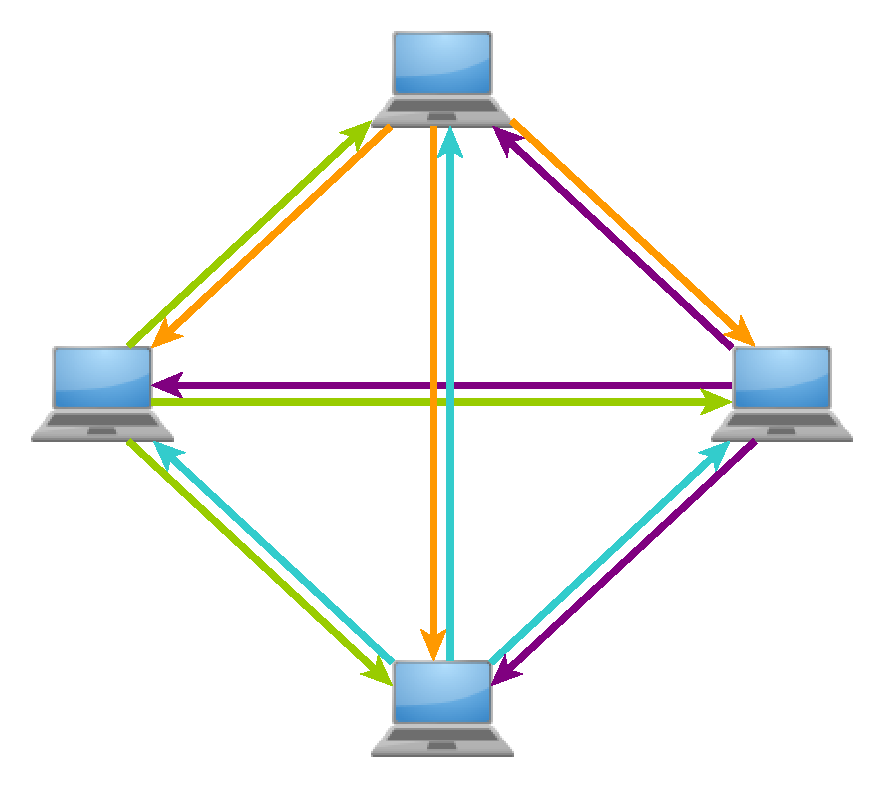
\includegraphics[width=\textwidth]{figures/dcomposite.pdf}
	\caption{Peer-to-Peer connections}
	\label{fig:p2p}
\end{minipage}
\end{figure}

	In this context, each client must only have one \emph{PeerConnection} to our streaming server and content shown to them is changed on demand either being it an individual or a composite view. This approach is centralized, as seen on figure \ref{fig:central}. Otherwise clients could follow a peer-to-peer connection, as seen on figure \ref{fig:p2p}, which would result on maintaining more connections and performing the composition of videos on client side.

	The composition of streams on client side is performed by receiving streams with the best quality possible but, due to undersizing the video of clients into a smaller region, this would result on wasting bandwidth on a quality that is not needed.

	Although the peer-to-peer approach could be used on our system, we conclude that we need to record the video on our streaming server because web clients have a very limited storage and peer disconnections may result on recorded video loss. 

	The same can be concluded to instant message delivery, each client must have only one \emph{WebSocket} connection to the application server which consequently relays the messages to other users.

	Relaying instant messages from clients through the our web servers is easier if all clients are connected to the same server because all messages can be directly delivered without sending messages across multiple web servers. 

	In the context of this thesis, we will not implement sending messages across web servers but, in order to allow our system to scale, we will consider that all conference participants are connected to the same server and our system is scaled by having conference rooms distributed across different servers.

\subsection{Software choices}

Furthermore, we have taken into account the compatibility between the streaming server, database and the operation transformation solutions, in order choose the appropriate framework to implement our web server.
%RP esta secção devia começar aqui, a explicar a escolha das tecnologias/produtos a usar em cada componente. O que tens antes são pormenores que só faz sentido discutir no final. Tens de ir sempre do mais geral para o mais detalhado.

As a result of our study about signaling protocols we have decided to exclude \ac{XMPP} due to the development difficulties that it exposes when using multiple web pages, namely the user re-authentication performed each time a page is loaded and the single tab usage limitation. As a consequence we have not chosen \emph{Jitsi Video Brigde} for stream processing as it uses \ac{XMPP}.

Accordingly, by excluding \emph{Jitsi Video Brigde} we have decided that our solution must use \ac{KMS}. Our web server could be implemented easily with \emph{NodeJS} or \emph{Java} due to the fact \ac{KMS} provides clients for both technologies. But others could also be used as \ac{KMS} also exposes their \ac{API} via \emph{WebSockets}.

Due to the fact we are going to use \ac{KMS} as streaming server solution, we could choose \emph{NodeJS} or any \emph{Java} based web framework for implementing our web application server. One of our criteria for choosing the web framework is the ability to follow the \ac{MVC} paradigm which can help us to organize our code. We have decided to implement our web server with the \emph{PlayFramework}\footnote{\url{https://www.playframework.com/}(acessed March 25, 2016)} using \emph{Java} because of our previous experience with it.

By default, \emph{Kurento Repository} is implemented over \emph{MongoDB}, for convenience our storage model will also use the same database.

Importantly, for the collaborative text editor, we have chosen \emph{OT.js} due to its server and storage implementation choice independence.

For the \emph{NAT Traversal} module, an \ac{ICE} server is not required to be on our infrastructure, as a public \ac{STUN} server can be used for testing our solution. Nevertheless, we recognize that for a production environment we would need to maintain our own \ac{TURN} servers in order to ensure connectivity to all clients.

Not less important, on the client computers, both \emph{Mozilla Firefox} and \emph{Google Chrome} could be installed as web browsers. As such, both should be supported. Libraries such as \emph{jQuery}, \emph{Bootstrap}, \emph{Adapter.js}, \emph{OT.js} can be downloaded from the web server and executed on the client side using any of these two browsers.
%RP relembrar que o IE e o Safari não suportam webrtc?

\begin{table}[H]
\centering
	\caption{Application Architecture}
	\label{table:apparch}
    \begin{tabular}{cccccccc@{}m{0pt}@{}}
	\hline 
\multicolumn{8}{|c|}{\cellcolor{Gray}Application}  &\\[12pt]\cline{1-5}\cline{7-7}
\multicolumn{1}{|c|}{jQuery} & \multicolumn{1}{c|}{HTML5} & \multicolumn{1}{c|}{CSS3 (Bootstrap)} & \multicolumn{1}{c|}{Signaling} & \multicolumn{1}{c|}{~~~~~ot.js~~~~~} & \multicolumn{1}{c|}{\cellcolor{Gray}~~~~~~~~~~~~~~~} & \multicolumn{1}{c|}{adapter.js} &   \multicolumn{1}{c|}{\cellcolor{Gray}~~~~~~~~~~~~~~~} &\\[12pt]\hline
\multicolumn{1}{|c|}{HTTP} & \multicolumn{2}{c|}{User Interface}  & \multicolumn{3}{c|}{WebSocket}    & \multicolumn{2}{c|}{WebRTC}      &\\[12pt]\hline
\end{tabular}
\end{table}

%RP acho interessante o que queres fazer aqui mas acho que está mal conseguido. A linha de baixo, devia ter coisas ao mesmo nível, o que não aconteçe.
% Qual a razão para HTTP estar por baixo do jquery e user interface estar ao lado?
% Sugiro colocar a applicação no meio e as várias interfaces (webrtc, websocket e http) uma de cada lado (esquerda, baixo e direita), indicando o que fica do outro lado (outro cliente, servidor web, servidor stream, etc)

Table~\ref{table:apparch} presents the application architecture and the underlying technologies seen from the user's perspective. \emph{Adapter.js} and \emph{jQuery} will ensure that our application is compatible with the most popular web browsers.
\emph{Bootstrap} will be used to make the user interface more appellative and responsive. With \emph{Bootstrap} it is quite easy to develop applications that adapt to mobile devices with different screen sizes.
%RP bootstrap não aparece na figura!

With respect to displaying content, the synchronization between multimedia elements will be performed through chains of \emph{JavasSript} events or by specifying the interval of time which time content must be visible. Other animations can be implemented with \ac{SVG} embedded on \ac{HTML}.
%RP Caiu do céu! Tens de explicar e ligar melhor a sequencia de texto

\section{Chapter Summary}
\label{architecture:summary}

In this chapter we have shown the modules needed in order to implement our solution.

Several technologies were taken into account for implementing each module, we have studied the pros and cons of each technology and decided the architecture for our solution.


